% Chapter Template

\chapter{Data Analysis and Methods} % Main chapter title

\label{Chapter:Data} 

%----------------------------------------------------------------------------------------

%----------------------------------------------------------------------------------------

Intro:\\
von den Rohdaten zur 3D VDF




\section{Data products}
Data in Form von 24-bit PHA words: Übertragungsrate Normal: 30 x 24 bit pro Spin\\

DPU selects a balanced ratio of high and low priority PHA: Details s. SWICS Paper Ende 3.2.2 (one-to-one basis?) \\

Voltage cycle: 64 steps, je ein Step pro spin, 1 Spin: 12 sec -> Duty Cycle 12.8 min
\\ \\
Tof: Range 10 -- 200 ns \\
1024 channels
resolution:
\\ \\
Ech: Range 40 - 600 keV \\
256 channels
resolution:
\\ \\
PHA words,\\
Channel numbers, EpQ mit Unsicherheit auftragen, EpQ \\ 
data transmission \\
SC bit rate? 1024 o. 512 bit/s


\subsection{Detection Efficiency, Doubles, Trebles}
(Frage Lars: Welche Wahrscheinlichkeit genau gibt die E. an? Ausgehend von einem Teilchen vor dem Instrument mit der richtigen Epq? Von einem Teilchen, das den EpQ Filter durchlaufen hat?)\\ \\
The detector efficiency is the probability to measure a particle that has entered the instrument(?). 
When working with SWICS, like for any physical measurement, one has to consider several effects that impede the ideal measurement as it is described in sec. todo. 
These effects are highly dependent on the ion species and deflection step and include for example that secondary electrons for the time of flight measurement (in carbon foil and SSD) may not be emitted properly. Also, ions could pass through the time of flight section on divergent trajectories due to scattering processes (in the carbon foil??). Possibly, the ion then does not hit the sensitive area of the SSD and does neither trigger a stop signal for the time of flight measurement nor a valid energy measurement in the SSD. Even for an ion that hits the SSD centrally

Another reason for a missing energy deposit in the SSD is that the ion's energy is smaller than the threshold of the SSD. The reason for choosing a nonzero threshold is to limit the influence of the SSDs natural noise. For SWICS this noise level is quite high (todo: Quelle!! Goldfolie?) so that the threshold is chosen to be TODO. Ions with a small mass and charge are most likely to not overcome the threshold. For $\mathrm{He^{+}}$ this is already the case for deflection step TODO that corresponds to a $\mathrm{He^{+}}$ velocity of TODO (s. sec TODO).
Unfortunately, $\mathrm{He^{+}}$ detection efficiencies are not known to us for Ulysses SWICS. Instead, we make use of the efficiencies from ACE SWICS (todo: woher?). As ACE SWICS uses different EpQ deflection steps and seems to have a different SSD threshold we extrapolated the values for Ulysses SWICS.
For the highest EpQ value TODO we interpolated the efficiency from the ACE triple efficiencies and then extrapolated linearly to an efficiency of 0 at EpQ step 17. By this, we accommodate for the fact that $\mathrm{He^{+}}$ does not have enough energy to deposit energy above the SSD threshold at step TODO and thus, the probability for a triple coincidence is zero (Todo: Verweis auf anderes Kapitel: Coverage). $\mathrm{He^{+}}$ efficiencies from ACE SWICS and the resulting efficiencies used for Ulysses SWICS are shown in fig. TODO. For sure, these values are not realistic but represent the overall trend of a decreasing efficiency for higher EpQ steps at least.


\subsection{Priority weighting}
SWICS performs an on-board mass and mass-per-charge-classification. For every ion with valid measurements the $m$ and $mpq$ are calculated based on the measurements of ESSD, Tof and the particle's EPQ-step using a look-up-table technique.\\
On the one hand these values are used for sorting the ions into predefined boxes in the m-mpq-space which yield in the so-called matrix rate, a second data product that is provided by SWICS.\\
Secondly, and more important for our analysis, the m and mpq information is used to sort every measured ion into one of three priority ranges.

Range, BRW\\ \\
\begin{tabular}{c|c|c}
	%\hline
	Range 0 & $m < 8.7$;  $m_0 : mpq < 3.3$ & $\mathrm{H}$, $\mathrm{He^+}$, $\mathrm{He^{2+}}$; Doubles\\ 
	\hline 
	Range 1 & $m > 8.7$ & Heavier ions \\ 
	\hline 
	Range 2 & $m_0 : mpq > 3.3$ & Doubles \\ 
	%\hline 
\end{tabular} 

%
%
%

\section{ET matrices, identification}
Fig. \ref{fig:et_matrix} shows longterm PHA data collected with Ulysses SWICS over two years for energy-per-charge step 25 (which is $10.05\,\mathrm{kV}$). For every particle with valid measurements the $\mathrm{E_{SSD}}$ channel is plotted over the ToF channel. As a particle's mass and mass-per-charge is connected to the measured values $EpQ$, $\tau$ and $E_{SSD}$ by equations \ref{eq:swics_set1} --  \ref{eq:swics_set3}, every ion species occupies a distinct position in the so-called \textit{ET-Matrix}. (Counts of different ion species sum up at distinct places in ... space.)


\begin{figure}[h]
	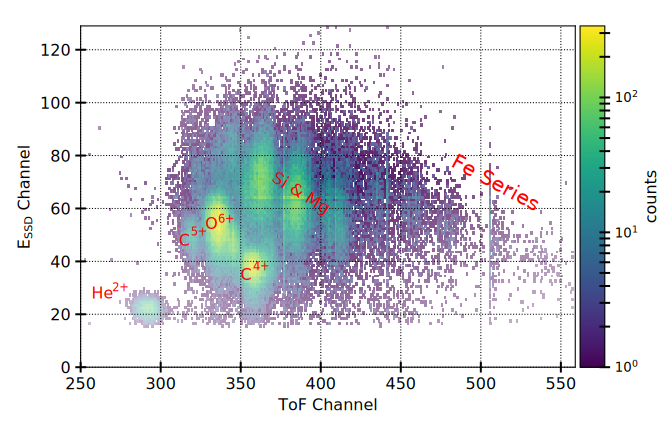
\includegraphics[width=0.9\textwidth]{Figures/et_matrix.pdf}
	\centering
	\caption{test}
	\label{fig:et_matrix}
\end{figure}


\subsection{Filter He+}
nominal w based on vsw -> solar wind ions rausfiltern
\begin{figure}[h]
	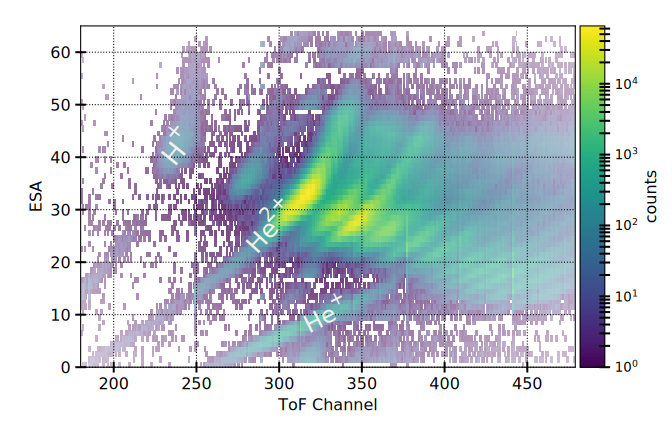
\includegraphics[width=0.9\textwidth]{Figures/epq_all.pdf}
	\centering
	\caption{test}
	\label{fig:epq_all}
\end{figure}


For extracting only the $\mathrm{He^{+}}$ events from the PHA data we plot the events' energy-per-charge over their measured ToF. 
Teilchen derselben mpq werden auf Kurven $todo$ geortet. Spezies höherer Mpq finden sich auf Kurven mit größeren ToF-Werten. Man kann so z.B. todo, todo und todo identifizieren. Unten ist He gut zu erkennen weil suprathermal. An die suprathermalen $\mathrm{He^{+}}$-Teilchen schließen sich zu höheren ToF andere Teilchen mit derselben mpq auf der gleichen Kurve an. Weil die Kurven dort enger liegen, kann man He in dem Bereich auch nicht von anderen mit ähnlicher mpq unterscheiden.
We can take advantage of SWICS' on-board priority weighting. We only plot the Range0-events. This roughly cuts out events with $m>8.7$. Nur H, He2+, He+ bleiben übrig als prominente Ionen. Man sieht, dass auch einige schwerere in die Box reinlecken, aber das betrifft nicht die ESA-Steps, in denen Helium auftritt.\\
Man kann jetzt prima per Auge eine Maske legen. Zusätzlich w filtern um eventullen Hintergrund zu unterdrücken...?
Man sieht, dass wir nur Helium-PHAs bis EpQ-Step todo auswerten. Der Grund ist, dass He1+ aufgrund der geringen Masse nicht genug Energie hat, die Triggerschwelle des SSDs zu überschreiten. Somit liegen He1+-Ionen bei höheren ESA-Steps (kleineren Energien pro Ladung) als Double Coincidences vor und taugen nicht für unsere Analyse.
\\
Für alle Jahre. Anzahl: todo
\\ \\
Plots: Nur RNG0, He und He2 gefiltert. In einem (dann nochmal und Fabrsala synchron) oder einzeln?
\\
Irgendwo He+, He++ und Protonen markieren


\subsection{Filter He2+}
für die spätere Kalibrierung (todo: Verweis) brauchen wir eine Spezies, bei der wir davon ausgehen, dass sie sich mit dem SW-Bulk bewegt und die als Triple Coinzidences vorliegt (für die Richtungsinformation). We choose He2+ wegen guter Statistik und auch in Range0. Im Gegensatz zu He1+ auch bei höheren ESA-Steps anzutreffen, weil mehr Nachbeschleunigung durch die höhere Ladung. Dadurch nicht so schnell unter SSD-Threshold. Gleiches Verfahren, einfach ausschneiden. Hier ist es nicht so wichtig, alles mitzubekommen, weil wir anhand von He2+ keine Analyse der VDF durchführen wollen. 
\\
Für alle Jahre. Anzahl: todo
\\ \\
Weitere Daten: vsw von SWOOPS, B-Feld
\\ \\
wie viele Daten bleiben über, wie viele PHA-Worte ca. pro Spin?
\\ \\
wohin damit? \\ \\
PHA pro Spin...
Ideal / mit Fehlern alpha, beta
\\ , Pile-up, random coincidences/ Schmutztail durch hohe Flüsse
\\
SWICS provides two types of data products from the analogue signals Tof, ESSD and the EPQ-Step.
24-bit
%
%
%






\section{Coordinate Systems}
For orientation bla we need coordinate system bla...

%
\subsection{Ulysses trajectory, HG system}
\textbf{Todo: Hinweis auf Zeichnung und Kapitel vorne}\\
Trajectory data is used from \citet{ulysses-data-archive} where Ulysses position data on a daily basis is available. The trajectory data is given based on different coordinates, including the heliographic coordinate system in the B1950.0 epoch.
\\ \\
Heliographic Coordinate System:\\
The heliographic (HG) coordinate system is a Cartesian Sun-centered system with the Sun's equatorial plane as a reference plane. Its X-axis is directed along the line of ascending node, which is the intersection line of the ecliptic and the solar equatorial plane. While the solar equatorial plane has an inclination of $i_\odot 7.25 ^\circ$ against the ecliptic \citep{fraenz_harper} the line of ascending node is at a longitude of $\Omega_\odot \approx 75^\circ$ relative to the First Point of Aries in 1950 \citep{nasa-earth-coord}. The Z-axis of the HG coordinate system is directed along the Sun's spin axis (northward) and the Y-axis completes the right-handed system. \\
In HG spherical coordinates the longitude $\varphi_{HG}$ is defined to be $0^\circ$ for directions along the X-axis and increases towards the Y-axis. The latitude $\vartheta_{HG}$ is $0^\circ$ for direction within the solar equatorial plane and $+90^\circ$ for northward directions.\\ \\
%
%
When working with the Ulysses trajectory data it was found that these data were given in spherical coordinates for which the $\varphi_{HG} = 0^\circ$ direction was towards $\sim -105 ^\circ$ longitude relative to the First Point of Aries. This means that the Ulysses trajectory coordinate system is shifted $180^\circ$ around the solar spin axis against the classical definition (s.a.).\\
In fig. \ref{fig:traj} Ulysses' spherical HG coordinates as well its distance from the Sun are given over the time of nearly the complete mission.


\begin{figure}[h]
	\includegraphics[width=1\textwidth]{Figures/HG_coord.pdf}
	\centering
	\caption{Ulysses trajectory data from November 1990 to June 2009 based on the data from the \citet{ulysses-data-archive}. Color shaded are the three orbits of the mission. \textbf{Above:} Shown is Ulysses' radial distance R from the Sun. Perihelion and aphelion of Ulysses' elliptical orbit can clearly be seen as the nearest/farthest distance of $1.3\,\mathrm{AU}$ and $5.4\,\mathrm{AU}$. Ulysses passes each of these points every 6.2 years and three times in total over the duration of the mission. \textbf{Below:} Shown are Ulysses' heliographic (HG) longitude and latitude. Note, that the longitude is shifted around $180^\circ$ with respect to the classical definition (s. text for details). A clear periodicity over Ulysses' three orbits can be seen. Maximum and minimum latitude are $\sim \pm 80^\circ$. These points are highest above the poles of the sun and are reached a few weeks before and after Ulysses' pass through the perihelion.}
	\label{fig:traj}
\end{figure}

\subsection{RTN Coordinate System}
Umrechnung von HG in RTN?
\\ \\
TODO:
The orbit itself is described in heliographic coordinates, so a cs that is constant (stable?) with respect to the sun. For describing positions and velocities in the frame of the spacecraft (e.g. AA) we need another cs...

\begin{figure}[h]
	\includegraphics[width=1\textwidth]{Figures/RTN_AA_angles.pdf}
	\centering
	\caption{Graphical representation of the RTN coordinate system (not to scale). Shown are the Sun (yellow), the Earth (blue) and the Ulysses spacecraft at a non-specific position on its orbit. $\vec{R}$ is defined as the unit vector along the line-of-sight Sun--Earth, $\vec{T}$ as the normalized cross product $\vec{\omega} x \vec{R}$ with $\vec{\omega}$ the angular velocity of the Sun (yellow vector). $\vec{N}$ completes the right-handed Cartesian system. Also shown is the definition of the aspect angle components $\varphi_{\mathrm{asp}}$ and $\vartheta_{\mathrm{asp}}$ as they are used in this work. The grey plane depicts the $\vec{R}$--$\vec{T}$ plane. $0 ^\circ < \varphi_{\mathrm{asp}} < 90^\circ$ and $-90 ^\circ < \vartheta_{\mathrm{asp}} < 0^\circ$ in the shown situation. \textbf{TODO: Zeichnung anpassen: Vektorpfeile, Indizes Winkel; Quelle Ulysses Dingsi}}
	\label{fig:rtn}
\end{figure}


For dealing with Ulysses' trajectory data it is useful to work with \textit{radial-tangential-normal} coordinates. The RTN coordinate system is defined relative to a moving object in the heliosphere -- in this case the spacecraft, Ulysses, and is centered at the sun. A graphical representation on the system can be found in fig. \ref{fig:rtn}. The unit vectors are $\vec{R}$, $\vec{T}$ and $\vec{N}$, where $\vec{R}$ points radially outward from the sun to the current position of the spacecraft. $\vec{T}$ is defined as the normalized cross product of the Sun's angular velocity $\vec{\omega}$ and $\vec{R}$. $\vec{N}$ completes the right-handed Cartesian coordinate system. Consequently, the RTN system is not defined for a spacecraft's position right above one of the Sun's poles as the cross product $\vec{\omega} x \vec{R}$ is zero here. Nevertheless we do not have to worry about this fact as not even Ulysses crosses the poles directly (todo: Verweis?).




%
%
%
\section{Collimator/Detector model}
\begin{figure}
	\centering
	\begin{subfigure}{.5\textwidth}
		\centering
		\includegraphics[width=1\linewidth]{Figures/col_single_new.pdf}
		\caption{A subfigure}
		\label{fig:sub1}
	\end{subfigure}%
	\begin{subfigure}{.5\textwidth}
		\centering
		\includegraphics[width=1\linewidth]{Figures/col_vspace_normal.pdf}
		\caption{A subfigure}
		\label{fig:sub2}
	\end{subfigure}
	\caption{A figure with two subfigures}
	\label{fig:test}
\end{figure}
\begin{figure}[h]
	\includegraphics[width=0.5\textwidth]{Figures/col_shells.pdf}
	\centering
	\caption{TODO}
	\label{TODO}
\end{figure}
Schreiben, dass das eigentlich von ACE/Lars kommt

\subsubsection{Motivation}
Kollimatormodell -- warum eigentlich -- wie umgesetzt?\\ \\
Das Ziel ist, einem gemessenen Teilchen einen v-Vektor zuzuordnen. Eine Sek-Det-Kombi ist aber nicht eindeutig. Ihre Bedeutung hängt davon ab, wohin das Instrument guckt (FoV), von der Eigengeschwindigkeit des SC und davon, wie das SC gerade gedreht ist. Zusätzlich hat der Kollimator eine komplizierte Geometrie, sodass eine analytische Lösung schwierig ist: Also numerische Lösung. \\
Was macht das Modell? -- Ich will das FoV zu jedem Zeitpunkt bestimmen. Ich nehme dafür einzelne Messpunkte auf der originalen Geometrie. Dann gebe ich noch ins Modell, wie das gerade ausgerichtet ist.\\
Berechnet anhand des AA, wohin Sun trigger schaut, wenn getriggert wird und rotiert coll. an entsprechende Position für Sek 0. Ordnet entsorechend andere Sektoren an.
Simuliert FoV durch Punkteraster \\
\subsection{Construction} \label{subsec:construction}
For reconstructing the velocity space that SWICS measures we need to know about the directions of incident particles that can enter the instrument.
\\ \\
The original geometry of the SWICS entrance system, in particular the collimator, was read out from a technical drawing \textbf{\textbf{(TODO: Quelle?!})}
Can be described as:
Width: Cutting out a hollow piece of 90 deg longitude (\textbf{todo: latitude? 4 grad?}) from a sphere (\textbf{of r ca. 26 cm ??}) at .. deg polar latitude. The piece is not flat but curved and has a height of ca. 5 cm. This geometry leads to two deflection plates that are curved but have a constant distance of ca. 3.7 cm over a relatively large area which is necessary to provide a constant voltage for the EpQ filtering (s. \ref{sec:EpQ}). Resulting opening angles of the collimator are $69^\circ$ in width and $4^\circ$ in height. \textbf{Todo: Zeichnung/Abbildung?}\\
The instrument is mounted with one of the narrow side edges parallel to Ulysses' spin axis. When we define this edge to lie on the x-axis of a three dimensional Cartesian coordinate system, the collimator geometry can be reconstructed by revolving this edge for $90^\circ$ around a straight line that lies in the xy-plane with an angle of $56^\circ$ relative to the x-axis. \textbf{Todo: Zeichnung/Abbildung!} Every third of these $90^\circ$ is reserved as the opening angle for each of the three detector elements, that are described in \textbf{Todo}.  \\
The detector's field of view is the solid angle over which the detector is sensitive to incoming particles.
It can be represented by a set of outward directed normal vectors on the opening plane of the detector. In our model, we have a variable number of those equidistant vectors both along the width and the height of the detector opening. The real continuous field of view is modelled better with an increasing number of normal vectors that cover the opening. Each of these normalized vectors $\mathrm{\mathbf{f_i}}$ has a unique direction $\mathrm{\mathbf{f_i} = \begin{bmatrix}f_{x,i}\,f_{y,i}\,f_{z,i}\end{bmatrix}}'$ in position space. An example... \textbf{(TODO: Plot)}
\\
With a spin of the Ulysses spacecraft the fixedly mounted SWICS instrument is revolves as well around the spacecraft spin axis. Consequently, the field of view is revolved around the x-axis in fig todo. One revolution of SWICS is divided up into eight sectors per $45^\circ$ each (todo: Verweis auf Instrumentenkapitel oder Erklärung). As the spacecraft is spinning continuously, also the real field of view changes its rotation angle continuously.
For our virtual detector we model this by rotating the field of view gradually over n steps through every sector.\\
The integrated field of view over one spin then comprises TODO single vectors $\mathrm{\mathbf{f_i}}$ which are directed symmetrically around the spin axis (s. Abbildung TODO)). In fig. Todo is shown the FoV of todo , you can see a shell with radius 1 bla...
\subsubsection{From FoV to Vspace}
The detector's velocity acceptance can be calculated by combining the directional information from the field of view and the value of absolute velocity from the current EpQ step. 
\\
A particle can only enter the detector when its absolute velocity is within the acceptance of the current EpQ step and when its inverted direction is within the detectors field of view. For a given acceptance velocity $v_i$ and a single field of view vector $\mathrm{\mathbf{f_i} = \begin{bmatrix}f_{x,i}\,f_{y,i}\,f_{z,i}\end{bmatrix}}'$ the accepted velocity is
\begin{align}
\mathbf{v_i} = \begin{bmatrix}v_{R,i}\\v_{T,i}\\v_{N,i}\end{bmatrix} = - \begin{bmatrix}f_{x,i}\\f_{y,i}\\f_{z,i}\end{bmatrix} \cdot v_i.
\label{eq:fov}
\end{align}
With consideration of the integrated field of view over one spacecraft spin (s. ), the acceptance velocity consists of the combination n\_todo discrete velocities which form a shell with radius $v_i$ in velocity space. (s. fig. TODO for v\_todo)




.
\\ \\
The central velocity for an ion of charge $q$ and mass $m$ for an energy-per-charge step $EpQ$ (in $keV/e$) is
\begin{align*}
\frac{v_c}{km \, s^{-1}} = \sqrt{\frac{2 \cdot EpQ \cdot 1.60217646\cdot10^{-19}\cdot |q|}{m \cdot 1.66053886 \cdot 10^{-27}} }
\end{align*}
with $m = 4 u$ and $|q| = 1$ for $\mathrm{He^{+}}$.\\
To represent the uncertainty in EpQ measurement, we take into account the relative uncertainty $\Delta \frac{E}{q}/\frac{E}{q} = \pm 5\%$ and translate it into an uncertainty $\Delta v / v = \frac{1}{2} \left( \Delta \frac{E}{q}/\frac{E}{q}\right) = \pm 2.5\%$ in accepted velocity. For every EpQ step we can now choose a number of $i_{epq}$ single velocities that are distributed evenly in the interval $\left[ v_c - \Delta v / v, v_c + \Delta v / v \right]$. The total number of accepted velocities $v$ is then $64 \cdot i_{epq}$.
\\
Different absolute velocities $v$ appear as distinct shells of radius $v$ in velocity space.
Ein Beispiel, der Übersichtlichkeit halber nur 3 Schalen, ist in bla gezeigt.
\\
With combining all $64 \cdot i_{epq}$ shells we obtain a dense three dimensional pattern of accepted velocities that simulate the real continuous velocity acceptance volume of the spinning detector.
\\ \\
When we measure a PHA word with a distinct SEC, DET and EPQ information, we can now determine its three dimensional velocity with our virtual detector. Of course, the resolution is limited as sector and detector areas are finite as well as the uncertainty $\Delta \frac{E}{q}/\frac{E}{q}$. By spreading the count over the entirety of velocity acceptances in the volume of the SEC DET EPQ combination, we take into account every velocity that could have led to this distinct PHA word.
\\ \\


.\\ \\ \\
Später schreiben, was für n verwendet wurden
\subsection{Eigen-velocity}
For the considerations in the previous section we assumed a detector on a spacecraft that is fixed in space. Obviously this is not the case for the Ulysses spacecraft (s. sec. TODO) which moves on its elliptical orbit around the Sun. \\
For determining the spacecraft's velocity we make use of the daily given trajectory data from sec. TODO. For every time stamp $t_i$ we calculate the spacecraft's instantaneous velocity by forming the differential quotient 
\begin{align*}
v_i = \frac{ \begin{bmatrix}v_{R,i+1}\\v_{T,i+1}\\v_{N,i+1}\end{bmatrix}_i  - \begin{bmatrix}v_{R,i}\\v_{T,i}\\v_{N,i}\end{bmatrix}_i} {t_{i+1} - t_i}
\end{align*}
with $t_{i+1}$ being the next time stamp, which is normally $t_i + 1\,\mathrm{d}$. Note, that the spacecrafts position at $t_{i+1}$ has to be considered in the RTN coordinate system that relates to the spacecraft's position at $t_i$. The resulting velocities in RTN coordinates are shown in fig. todo.
\\
--Bewertung Größenordnung--
\\
To correct the measured velocities for the spacecraft's eigen-velocity, we simply add the resulting velocity components to the velocity acceptance. Thus, for every time stamp the shells (s. fig todo) are shifted a bit in velocity space based on the respective eigen-velocity.


\subsection{Orientation of the Detector}
Until now we have assumed that Ulysses' spin axis is aligned with the R-axis of the coordinate system, i.e. that the spin axis points directly to the Sun. In fact, this is not the case in general. Due to telemetry reasons, Ulysses' high gain antenna has to be oriented directly towards Earth (todo: Vergleich mit ACE, warum?). As Ulysses' spin axis is aligned with the electrical axis of the antenna \citep{wenzel_ulysses}, has an offset towards the line of sight spacecraft-Sun. This offset is called \textit{aspect angle} and is a permanently changing quantity as a function of Ulysses' position and the position of the Earth. As a varying aspect angle results in SWICS covering different parts of velocity space it is essential to consider this quantity in detail.
%
%
\subsubsection{Calculation of the Aspect Angle}
\begin{figure}[h]
	\includegraphics[width=1\textwidth]{Figures/aa_new.pdf}
	\centering
	\caption{The evolution of Ulysses' aspect angle components $\varphi_{\mathrm{asp}}$ and $\vartheta_{\mathrm{asp}}$ from 1991 to the end of the mission are shown. The aspect angle is the angle between the line-of-sight Ulysses--Sun and the orientation of Ulysses' spin axis. A constantly changing aspect angle results from the fact that the spacecraft's antenna, that is nearly parallel with the spin-axis, has to point towards Earth all the time. Particularly large aspect angles occur during the three fast latitude scans around 1995, 2001 and 2007. Here, Ulysses' distance to Sun and Earth is at a minimum. \textbf{Also shown is the... (todo: raus aus der Zeichnung?)} }
	\label{fig:aa}
\end{figure}
The aspect angle is measured from the line-of-sight Ulysses--Sun (that is $\vec{R}$) to the line-of-sight Ulysses--Earth. To describe this angle uniquely for any moment, we need two spherical coordinates $\varphi_{\mathrm{asp}}$ and $\vartheta_{\mathrm{asp}}$ based on the RTN system. As shown in fig. \ref{fig:aa}, $\varphi_{\mathrm{asp}}$ is measured in the $\vec{R}$--$\vec{T}$ plane between $-\vec{R}$ and the projection of the line-of-sight from Ulysses to the Earth into this plane. $\varphi_{\mathrm{asp}}$  is $0^\circ$ for directions along $-\vec{R}$, that is the line-of-sight from Ulysses to the Sun and increases to positive values towards $-\vec{T}$. $\vartheta_{\mathrm{asp}}$ is the angle between the projection of the line-of-sight from Ulysses to the Earth into the $\vec{R}$--$\vec{T}$ plane and the line-of-sight itself. It is defined as $0^\circ$ for directions that lie within the $\vec{R}$--$\vec{T}$ plane and $+90^\circ$ for directions along $\vec{N}$.\\
(Todo: Lars fragen, ob die genaue Rechnung hier rein muss, Kladde S. 79)
For the calculation of the aspect angle we used the Ulysses trajectory data (Verweis ... TODO) and Earth trajectory data in heliographic coordinates on a daily basis from \citet{nasa-earth-coord} and converted both to RTN coordinates. In fig. \ref{fig:aa} both components $\varphi_{\mathrm{asp}}$ and $\vartheta_{\mathrm{asp}}$ as well as the \textit{flat} aspect angle $\alpha$ with  $\alpha = \arccos(\cos{\varphi_{\mathrm{asp}}}) + \arccos(\cos{\vartheta_{\mathrm{asp}}}) -1$ are shown over the time of the mission. $\varphi_{\mathrm{asp}}$ varies in the range from $\sim - 25^\circ$ to $\sim 42^\circ$ and $\vartheta_{\mathrm{asp}}$ in a range from $\sim - 30^\circ$ to $\sim 17^\circ$. Large angles occur especially around the three fast latitude scans, i.e. when Ulysses is at its perihelion and has the smallest distance to Sun and Earth.\\
(Todo? Beschreiben, dass ich $\alpha$ mit dem Datenprodukt SPE verglichen habe?)
\\ \\
\begin{figure}[h]
	\includegraphics[width=0.5\textwidth]{Figures/col_aa_marker.png}
	\centering
	\caption{todo}
	\label{fig:col_aa}
\end{figure}
steps asp Winkel

The variable aspect angle is incorporated into the analysis by rotating the field of view corresponding to $\varphi_{\mathrm{asp}}$ and $\vartheta_{\mathrm{asp}}$. This results in a likewise rotation of the velocity acceptance space. In fig. \ref{fig:col_aa} the acceptance velocity for a single absolute velocity $v = 600\,\mathrm{km\,s^{-1}}$ is shown for $\varphi_\mathrm{asp} = 25^\circ$ and $\vartheta_{\mathrm{asp}} = -10^\circ $. Note, that the orientation here seems to be mirrored against the convention that has been described before. This is due to the inversion when transitioning from the field of view to velocity acceptance, s. eq. \ref{eq:fov}.\\
When comparing fig todo with fig todo, where a situation with $\vartheta_{\mathrm{asp}} = \varphi_{\mathrm{asp}} = 0$ is shown, it becomes clear that especially larger aspect angles change the link between a distinct sector-detector element and a volume in velocity space. While with a zero aspect angle a radial velocity (along $\vec{R}$) would be detected right in the middle of the velocity shell and definitely in the innermost detector, this is not the case for the aspect angle in fig. todo. Here, an exclusively radial oriented velocity would be detected in a distinct sector in the central detector. (Andersrum bedeutet das, dass eine Sec-Det-Info nur zugeordnet werden kann, wenn die Ausrichtung des Detektors bekannt ist!)

\subsubsection{Probe}
For checking if the considerations made before are reasonable and if the virtual detector works in the right way, we want to have a look at data of which we believe to know the VDF. Appropriate test data is the solar wind itself as it is believed to flow radially outwards from the sun (Todo:Quelle). An ideal candidate within the solar wind is $\mathrm{He^{2+}}$ as the most abundant species (todo: Quelle). Thus, we can identify $\mathrm{He^{2+}}$ easily in fig Todo and are provided with good statistics. Unlike protons, which are even more abundant in the solar wind, $\mathrm{He^{2+}}$ most likely deposits energy above the detector's threshold in the SSD detector (s. chap Todo). This is because of its higher mass and the twice as high charge, which leads to a higher gain in energy by the post acceleration (todo:nochmal Verweis?). Only when a particle triggers an ESSD measurement (Triple Coincidence) we get a directional information about its velocity (Verweis todo). Protons are most often measured as Double Coincidences except for suprathermal protons, for which the assumption of radial stream must not hold true (Todo:Quelle). For selecting $\mathrm{He^{2+}}$ we proceed like described in chap. todo.
Wie viele PHAs sind das dann insgesamt und pro Jahr? Schreiben, dass das nicht so genau gemacht werden musste, weil keine VDF Analyse...
\\ \\
In a first step we look at periods of time in which both aspect angle components $\varphi_{\mathrm{asp}}$ and $\vartheta_{\mathrm{asp}}$ were small (Todo: genau?). For these nr\_todo PHA words we draw a histogram (??) of their sektor and detector information. The result can be seen in fig. todo. The histogram shows that mainly the innermost detector has counts. This is the expected behavior when we imagine the instrument on a spacecraft that points directly to the Sun. A radially streaming flow then hits the instrument's detector that is oriented sunwards. This does not change with the spin of the spacecraft. This result is also consistent with the detector model for $\varphi_{\mathrm{asp}} = \vartheta_{\mathrm{asp}} = 0$ which is shown in fig. todo. A radial stream can be represented here by the black line which cuts through the velocity shell in its center, the region of the innermost detector, bla. Irgendwie schöner schreiben...
(Due to the width... auf allen Sektoren?)
\\ \\
In a second step we take a look at a time period in which Ulysses had a substantial aspect angle. This is particularly the case for when Ulysses is near its perihelion, s. fig todo. We choose for the second orbit, i.e. days 1-90 (?) in 2001. For all $\mathrm{He^{2+}}$ PHA data from this time we again histogram sector and detector information, which is shown in fig. todo. Compared to fig. todo the maximum of counts is now shifted clearly towards a single sector (Nr.?) and the central detector. This is consistent with the virtual detector in fig. todo, where the aspect angle's quantity matches the one in the selected time period. With this orientation a radial stream from the Sun hits the instrument on its center detector and only while a particular moment (?!) of the spin/rotation (?!). Counts do not show up exclusively with this single sector-detector combination but slightly spread out over adjacent sector-detector elements. This is due to the fact that solar wind $\mathrm{He^{2+}}$ does not stream as an ideal beam but has a certain width (todo: Referenz).
\\ Verweis: Sektordetails im nächsten Kapitelchen

\begin{figure}[h]
	\includegraphics[width=0.5\textwidth]{Figures/hist_det_sec_aa_90days2001}
	\centering
	\caption{TODO}
	\label{TODO}
\end{figure}


\subsubsection{Sunpulse Trigger -- Rotation}
In the previous section hat man gesehen, dass sich die PHA Counts für einen großen AA auf den mittleren Detektor konzentrieren. In diesem Abschnitt soll geklärt werden, wovon es abhängt, in welchem Sektor der Schwerpunkt der Counts landet. 

As mentioned before (todo: ist es?), one SC spin is divided into 8 sectors, starting with sector 0 and ending with sector 7.
Every spin's start is defined newly by the \textit{spin reference pulse} of Ulysses \citep{hiscale}. 

This pulse is triggered by a combination of four sun sensors which detect when the Sun crosses a plane that is spanned by the spacecraft's spin axis and the spacecraft's x-axis, which is a particular axis perpendicular to the spin axis.
The spin reference pulse is not uniform over time as the position of the Sun relative to the spacecraft changes with varying aspect angle.\\
To extract correct directional information from a sector data product of an ion that has been detected by SWICS it is essential to know the relative orientation between SWICS' main axis and the x-axis on the spacecraft. In the virtual detector this is implemented as an angle against the line-of-sight spacecraft-sun by which the field of view is rotated around the spin axis.\\
From the \citet[][S.20-22]{swics_dpu} we know with \textit{normal orientation} the sun pulse occurs in the center of SWICS sector 4, which implies a $180^\circ$ offset between the line-of-sight spacecraft-sun and SWICS sector 0 (s. fig TODO). However, one can also read that it was possible to set a fine adjustment which would lead to an offset of the sun pulse from this center line up to $22.5^\circ$ \citet[][S.48]{swics_dpu}. Unfortunately, we do not know about the value that has been chosen.
\\
If we assumed a wrong angle, a particle beam coming from a fixed direction in a sun-fixed frame would be linked to a different direction. But this shift between true and supposedly measured direction is not constant over aspect angles. If we then measured over a longer time period with various aspect angles, we would measure the beam as blurred in velocity space.
\\
To make sure our model uses the right angle, we again choose $\mathrm{He^{2+}}$ as a test population of which we assume a beam-like behaviour streaming radially from the Sun. Also, we can only look at time periods when the aspect angles were large and the maximum of $\mathrm{He^{2+}}$ counts occurs in the central or outermost detector. Only here we can clearly discriminate between single sectors. When measured in the innermost detector the slightly widened distribution of $\mathrm{He^{2+}}$ would spread across all sectors as they are close together here (s. fig todo).
From fig Todo, where we histogrammed bla, we find that the overall idea of a sun pulse in sector 4 should be right when we believe the assumption that $\mathrm{He^{2+}}$ streams radially from the Sun. To check for a potential fine adjustment we search for tendencies of the maximum of counts sweeping to an adjacent sector.
\\
Zeigen: Für lange Zeiträume: $\mathrm{He^{2+}}$ kommt zentral. Für einzelne kurze: unterschiedlich.
Deshalb: grober Check von wegen Detektor geht gut. Für das Feintuning (180 Grad oder doch was anderes?) reichts aber nicht...
\\
Schemazeichnung SunPulser, dazu Problem irgendwie zeigen

\subsubsection{Übergang w}
Steps vsw
\\
With the considerations of eigen-velocity and orientation we can now use the virtual detector for displaying velocity distributions of $\mathrm{He^{+}}$ pickup ions. 

Mithilfe des virtuellen Detektors können jetzt geeignete (Triples) PHA Worte in dreidimensionale Geschwindigkeitskomponenten übersetzt werden (vorher: nur Betrag. Jetzt: Komponenten).
Erst mit diesen entfalteten Einzelkomponenten kann man den wichtigen Schritt gehen und in den Sonnenwindframe übergehen.
This is done for every PHA word (nein. jeder v-Akzeptanzpunkt in jeden getroffenen Sek-Det-Kombidings...) by subtracting the instantaneous solar wind speed in R-component from the ion's velocity in spacecraft frame: 
\begin{align*}
\mathbf{v_{i,sw}} = \begin{bmatrix}v_{R,i,sc}\\v_{T,i,sc}\\v_{N,i,sc}\end{bmatrix} - \begin{bmatrix}v_{sw}\\0\\0\end{bmatrix}
\end{align*}
In a last step every component of the resulting vector is divided the by solar wind speed:
\begin{align*}
\mathbf{w_{i,sw}} = \begin{bmatrix}v_{R,i,sw}\\v_{T,i,sw}\\v_{N,i,sw}\end{bmatrix} / \begin{bmatrix}v_{sw}\\v_{sw}\\v_{sw}\end{bmatrix}
\end{align*}
By this, the transition from velocity space in the spacecraft frame to solar wind independent w space in solar wind frame of reference is made.
%
%
%
\section{VDF}

%
\subsection{Velocity Space Coverage}
When analyzing $\mathrm{He^{+}}$ PUI w-spectra with Ulysses SWICS, several effects have to be considered that limit the observable part of w-space. The most obvious restriction results from the fixed geometry of the collimator (s. sec. \ref{subsec:construction})) which allows to observe only a dome-shaped part of the w-space when considering the spin of the spacecraft and varying EpQ steps. (However, this dome is not fixed in w-space for different orientations of the spacecraft.
While the ever changing aspect angle of Ulysses introduces a complex subject to directional data analysis it also enlarges the integrated coverage of velocity space over time.)\\
Furthermore, we have to deal with a limitation of the coverage in $w_R$-direction particularly for $\mathrm{He^{+}}$ triple coincidences. The observable EpQ range for $\mathrm{He^{+}}$ is limited to TODO to TODO, which corresponds to steps todo to todo. While A is the instrument's highest possible EpQ value, B is the lowest value for which $\mathrm{He^{+}}$ still has enough energy to overcome the energy threshold of the SSD and thus can trigger a valid energy measurement. 
The w-range that is consequently covered is highly dependent on the prevalent solar wind speed. For $v_{sw} = 700 \,\mathrm{km/s}$ the absolute w in a spacecraft frame is limited to TODO. For slow solar wind at $v_{sw} = 300 \,\mathrm{km/s}$ todo... . 
That means that we are limited to time periods with fast solar wind as we do not expect to measure the bulk of $\mathrm{He^{+}}$ PUI at w größer als... TODO. In fig. TODO an exemplary w-space coverage for vsw = Todo and no aspect angle is sketched.
\\ \\
Evtl. woanders hin und irgendwie besser schreiben: \\
In fig. \ref{fig:vsw_years} a histogram for occurring solar wind speeds is shown -- limited to times in which $\mathrm{He^{+}}$ triple coincidences were measured. Measured with SWOOPS. The number on the right indicates the total number of $\mathrm{He^{+}}$ PHA triple coincidence data that was received for that year. One can see the overall variation of the solar wind speed (due to different latitude: slow/fast sw) and that the total number of received data decreases heavily towards years in which Ulysses approaches the orbit's aphelion. This is mainly an effect of pickup ion flux reduction that scales with $r^{-2}$ due to the expansion of the solar wind (Todo:Quelle?).
\begin{figure}[h]
	\includegraphics[width=0.9\textwidth]{Figures/vsw_all_years_brw.pdf}
	\centering
	\caption{TODO... u.a.: norm; pad links neu}
	\label{fig:vsw_years}
\end{figure}


%
\subsection{Phase Space Normalisation}
We are now able to combine the information about sector, detector and EpQ step from the selected $\mathrm{He^{+}}$ PHA triple coincidences with the information about how the spacecraft was moving and which direction it was facing at the time of the measurement.
Counts that we have collected over a certain time period can be mapped into three dimensional w-space by this. However, for deriving physical quantities from these, a transition from counts to phase space density has to be made.\\
Firstly, we consider a single spin of the spacecraft, which normally corresponds to one EpQ step of SWICS.
Counts $N_{jk}$ that have been measured in a phase space volume that has been covered by a sector-detector element $j$ during the EpQ deflection step $k$ can be connected to the average phase space density $\delta_{jk}$ in this volume by an integration over the three dimensional velocity space:


\begin{align*}
N_{jk} &= \iiint\displaylimits_{v_{\varphi j}v_{\vartheta j}v_{R k}} \rho_{jk}	V_k	\,\,	d^3v,
\end{align*}
where $V_k = G \, \tau \, v_k$ is the spatial volume of the measurement with the geometrical factor $G = 0.0225 \,\mathrm{cm^2}$ (TODO: Quelle. Bei gloeckler steht das nicht?), $\tau = 12/8\,\mathrm{s} = 1.5\,\mathrm{s}$, the time of the measurement in a single sector and $v_k$ the central velocity for $\mathrm{He^{+}}$ in the EpQ step $k$ (Todo: Plot, Formel? Und dann Verweis nach vorne).
With the opening angles of a single sector-detector element of $4^\circ$ in width and $69^\circ /3 = 23^\circ$ in length and the height of this element $\Delta v_k$ we can write
\begin{align*}
%&= \iiint\displaylimits_{v_{\varphi i}v_{\vartheta j}v_{R k}} \rho_{ijk} \,	G \, v_k \, \tau	\,\,	d^3v \\
N_{jk} &= v^2_k \left(\frac{\pi^2}{180^2}\cdot4 \cdot 23\right) \, \Delta v_k \, \rho_{jk} \,	G \, v_k \, \tau.
\end{align*}
$\Delta v_k$ is determined by the uncertainty in EpQ measurement. It has been found to be $\Delta v_k = 0.025 \, v_k$ in sec. todo:chaptr FoV to vspace, which gives us
\begin{align*}
N_{jk} &= v^4_k \left(\frac{\pi^2}{180^2}\cdot4 \cdot 23\right) \, 0.025\, \rho_{jk} \, G  \, \tau.
\end{align*}
This we can rewrite with the phase space volume $V_{k}$ as 
\begin{align*}
\rho_{jk} &= \frac{N_{jk}}{V_{k}}.
\end{align*}
Notice, that $V_{k}$ is only dependent on the EpQ step $k$, as the sector-detector elements span the same (absolute) phase space volume for one EpQ step.\\
When we want to measure more than one spin, it has to be considered, that the probability to detect an ion is dependent on the EpQ step. This behaviour can be described by the detection efficiency.
\\ \\
The detection efficiency can be considered in phase space normalisation by weighting the spanned phase space volume for every sector detector element with the efficiency of the respective EpQ step: 
\begin{align*}
\rho_{jk} &= \frac{N_{jk}}{V_{k}\cdot eff_k}.
\end{align*}
As the instrument covers different phase space volumes with varying aspect angle, changing parts of phase space volume are covered.
However, we are actually interested in the average phase space density at a distinct volume element in phase space. This we get by dividing the counts in the volume element $v_i$ by the measured volume, both integrated over time and this volume. This means that we consider the time in which we we could have measured blaaaa.
\begin{align*}
\rho_{v_a} = \frac{\iint\displaylimits_{t\,v_a} N \, dv dt}{\iint\displaylimits_{t\,v_a} V\,eff\,dv dt}
\end{align*}




%.
%\\ \\ \\
%Mittlere Phasenraumdichte in einem Bin, in den zwei Instrumentenbins A und B reingehen:
%(differential PSD)
%\begin{align}
%\bar{\rho} = \frac{N_A + N_B}{\frac{N_A}{N_{A,ges}} V_A + \frac{N_B}{N_{B,ges}} V_B }
%\end{align}
%Dabei ist $N_i$ die Anzahl der Hits, die im Messbin gelandet sind und $N_{i,ges}$ die gesamte Anzahl an Bins. Hits heißt GEsamtcounts durch Detektoranzahl. Eigentlich gebe ich statt $N_i$ $N_i \cdot Detektoranzahl$ rein, aber das kürzt sich ja raus.\\ \\
%Effizienz und Sektorgewichte dazu:\\
%Allg.:
%\begin{align*}
%\rho = \frac{N \cdot brw}{V \cdot Eff}
%\end{align*}
%Und dann
%\begin{align}
%\bar{\rho} = \frac{N_A + N_B}{\frac{N_A}{N_{A,ges}} \frac{V_A \cdot eff_A}{brw_A} + \frac{N_B}{N_{B,ges}} \frac{V_B \cdot eff_B}{brw_B} }
%\end{align}








